\section{Curvature}
\label{sec:curvature}

In this section, we discuss smooth and discrete curvature. There are several
equivalent definitions of curvature. There are tradeoffs between them,
some are more intuitive while others lend themselves to efficient computation.
First, we warm up with curves in the plane, then move to curves in $\R^3$.
Then, we consider curvature for surfaces, both smooth and polygonal.
Finally, we define Gaussian and geodesic
curvature, two key terms of the Gauss-Bonnet theorem.

\subsection{One Dimensional Curves}

What do we require of a definition of curvature of a one dimensional curve
in the plane? We would like a number the represents how 
different a curve is from a straight line.
A straight line should have zero curvature and the unit circle should have
curvature one. Moreover,
 large circles should have less curvature than smaller circles.
Ideally, definition should also differentiate between
curving to the left and curving to the right.


For any point on a smooth one dimensional curve in the plane,
we can approximate the curve with a circle.
The best approximating circle is called the  \EMPH{osculating circle}.
A natural definition of the \EMPH{curvature} is the inverse of the radius of the osculating
 circle $k=\frac{1}{r}$.
See \figref{osculating-circle} for an example.
The osculating circle meets the requirements for a definition of curvature as long
as we allow the straight line to have an osculating circle with infinite radius.
We determine the sign of the curvature by which side of the curve the osculating circle is on.
However, computing the radius of an osculating circle is some what cumbersome (Exercise 1).

\begin{figure}[htb]
	\centering
	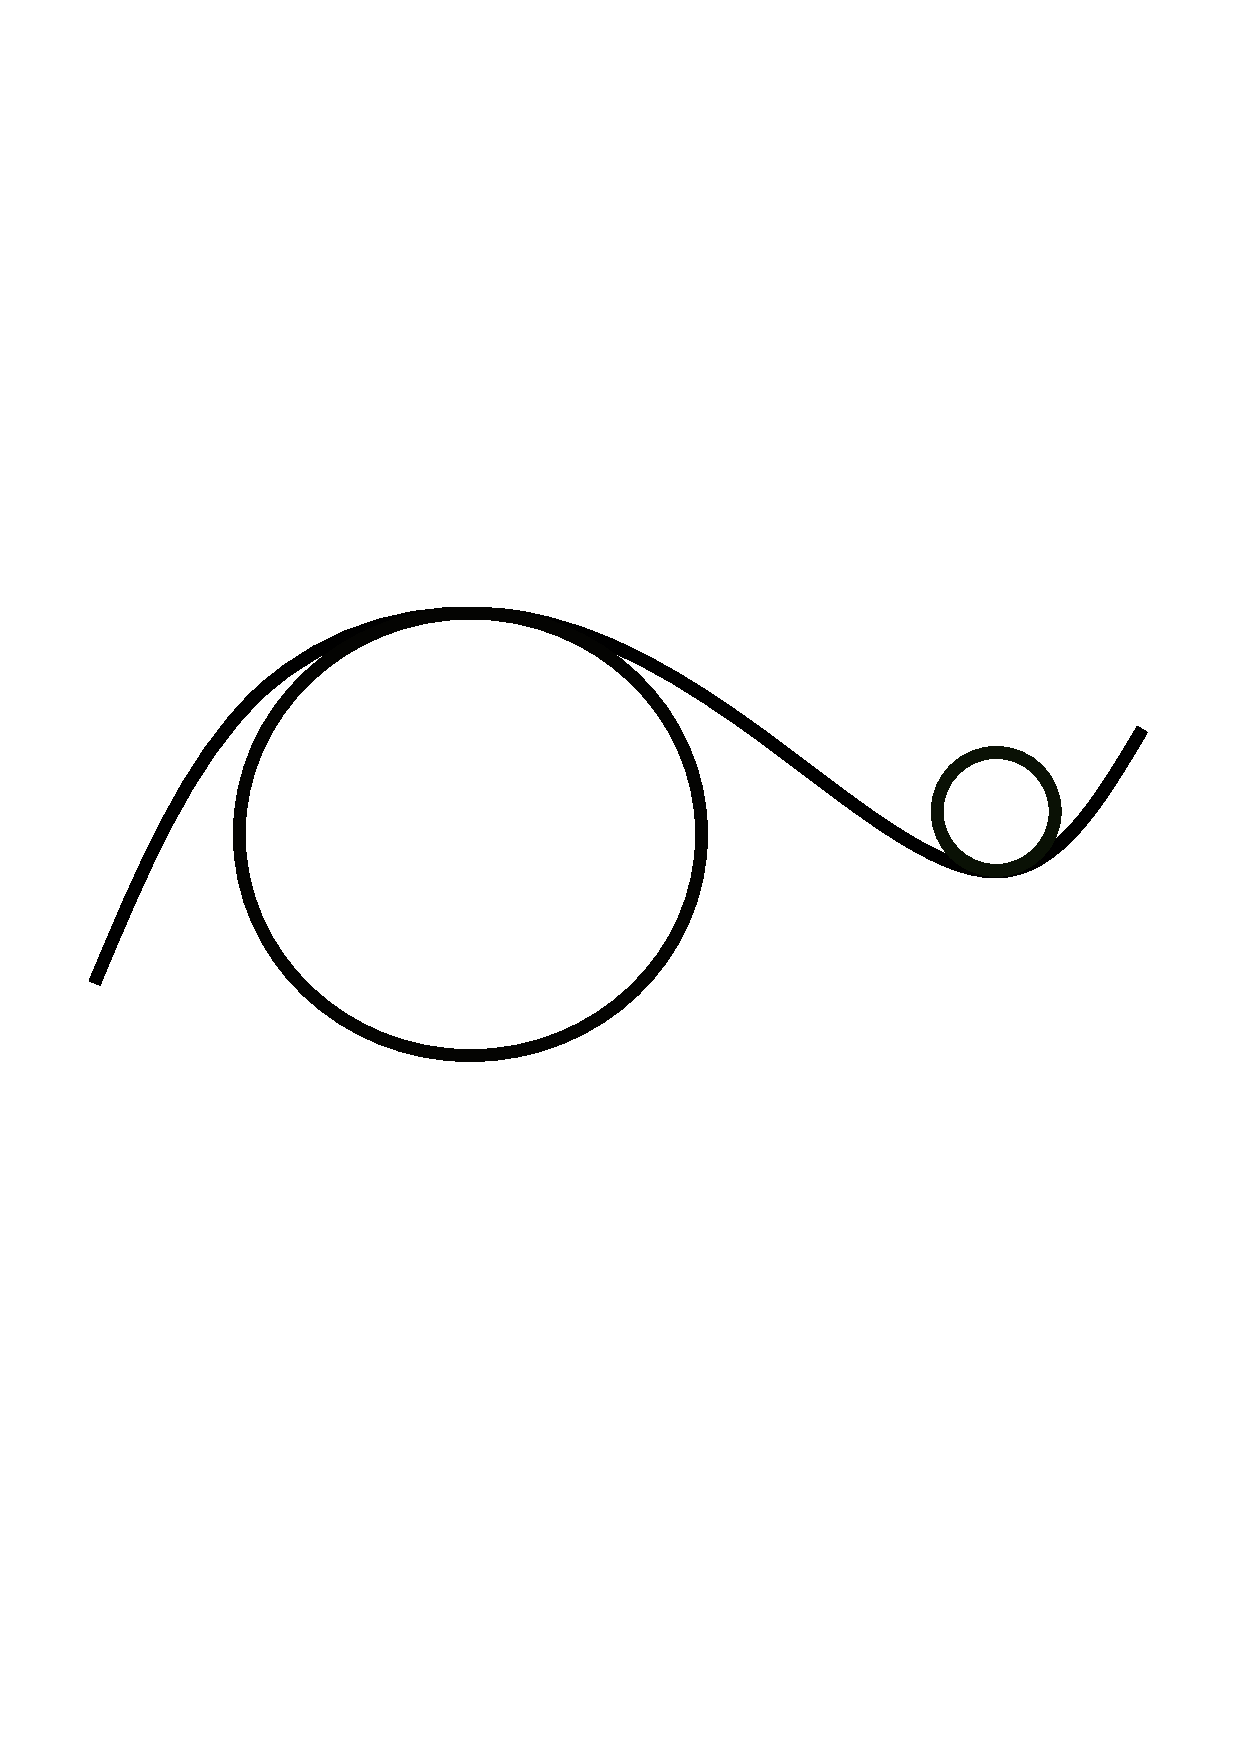
\includegraphics[width=.3\textwidth]{curvature/osculating}
	\caption{A curve with two osculating circles. The curvature at these points
	have opposite sign.}
	\label{fig:osculating-circle}
\end{figure}

Often curves in the plane are parameterized, for example
the circle of radius $r$ in the plane can be parameterized by
$$c(t)=(r\cos(t),r\sin(t))$$
 for $t\in [0,2\pi]$ is a curve in the plane.
If a curve is differentiable, another interpretation of curvature 
is the rate of change
of the angle between the curve and its tangent vector. 
We do not want this
rate to depend on how fast we are traversing the curve, one way to standardize
the speed is to parameterize by arc length, meaning the $t$ in  represents 
the distance traveled along the curve, in this case, the arc length parameterization
of the circle with radius $r$ is $$C(t)=\left(r\cos\left(\frac{t}{r}\right),r\sin\left(\frac{t}{r}\right)\right).$$

The rate of change of the angle between a curve and its unit tangent vector $T$, is the magnitude
of the derivative of $T$, see \figref{smooth-tangent}. Curvature is then
\begin{equation} \label{eqn:kappa}
\kappa= \pm | T'(t)|.
\end{equation}
where $t$ is arc length.  


For the circle of radius $r$ we have,
$$T(t)=\left(-\sin\left(\frac{t}{r}\right),\cos\left(\frac{t}{r}\right)\right)$$
and 
$$|T'(t)|=\left|\frac{1}{r}\left(-\cos\left(\frac{t}{r}\right),-\sin\left(\frac{t}{r}\right)\right)\right|$$
so
$$\kappa(t)=\frac{1}{r}.$$
We see that,  at least in this case, our definition of curvature in \eqnref{kappa} agrees with the
osculating circle definition. 
For a plane curve $\gamma(t)$ we can summarize above computation as
\begin{equation} \label{eqn:kappa1}
\kappa(t)=\frac{|\gamma'(t)\times \gamma''(t)|}{|\gamma'(t)|^3}.
\end{equation}

What about discrete curves in the plane? A discrete curve is a sequence of connected
line segments. Where two
segments meet there is a sharp corner. The curvature of a point in the interior of a segment
is zero. But what about the corners? Is there a well defined osculating circle? The tangent
vector is not defined!
Consider the exterior angle formed by extending one of the segments, as in \figref{discrete-plane}. 
If the segments are colinear, then the exterior angle is zero. If the interior angle
is smaller, then the curvature is greater as desired.




\begin{figure}[htb]
    \captionsetup[subfigure]{justification=centering}
    \centering
    \begin{subfigure}[b]{0.35\textwidth}
        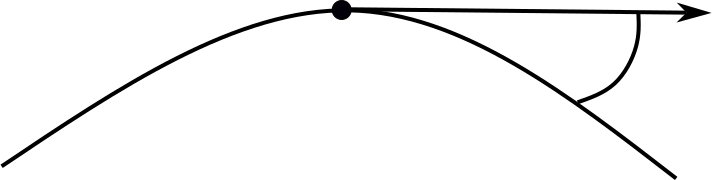
\includegraphics[width=\textwidth]{background/interior-angles-triangles}
       \subcaption{}\label{fig:smooth-tangent}
    \end{subfigure}
        \hspace{1cm}
        \begin{subfigure}[b]{0.35\textwidth}
        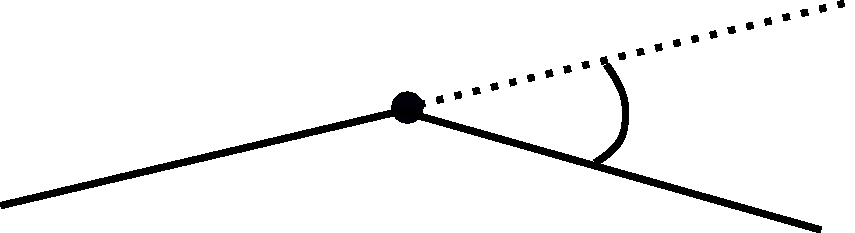
\includegraphics[width=\textwidth]{background/discrete-plane}
        \subcaption{}\label{fig:discrete-plane}
        \end{subfigure}
    \caption{(\subref{fig:smooth-tangent}) The tangent vector of a curve in the plane at a point.
        (\subref{fig:discrete-plane}) The exterior angle on a discrete curve in the plane.
    }
    \label{fig:osculating-sphere}
\end{figure}







What about curves in $\R^3$? Now there is another dimension, we can curve in the plane
and `twist' vertically out of the plane.
This additional freedom is called torsion.
Let $\gamma(t)=(x(t),y(t),z(t))$ be a smooth curve in $\R^3$.


We traverse $\gamma$
at unit speed so that the length of the velocity vector is one, $\gamma'(t)^2=1,$ and by the chain rule, $\gamma'\cdot \gamma''=0$.
This implies $\gamma'$ and $\gamma''$ are orthogonal.
Thus, the
vector $\gamma''=N$ is normal to the $\gamma$. 
By taking the cross product of $N$ and $T$ we obtain a vector $B$ called
the binormal vector.
The vectors $T,N$ and $B$ form the \EMPH{Fernet frame} of $\gamma$ a $p.$


The rate of change of the tangent vector is the curvature and the rate of change in
the binormal is the torsion. If the curve is a straight line for part of the parameterization,
then the Fernet frame is not well defined. We leave it to the reader to think about how to handle
this case.

\subsection{Curvature of Surfaces}


Moving up a dimension, let us now consider how to measure
the curvature at a point on a surface. As with curvature in the plane,
there are several equivalent ways to define curvature.
 The osculating-circle idea can be adapted
 to  surfaces in $\R^3$ by considering the \EMPH{osculating sphere},
But notice that at a saddle point on a surface it is not clear which sphere
best approximates the surface. See \figref{osculating-sphere} for two
equally reasonable ways to approximate a saddle with a sphere.

\begin{figure}[htb]
    \captionsetup[subfigure]{justification=centering}
    \centering
    \begin{subfigure}[b]{0.25\textwidth}
        \includegraphics[width=\textwidth]{curvature/sphere-above-saddle}
       \subcaption{}\label{fig:sphere-above-saddle}
    \end{subfigure}
        \hspace{1cm}
        \begin{subfigure}[b]{0.25\textwidth}
        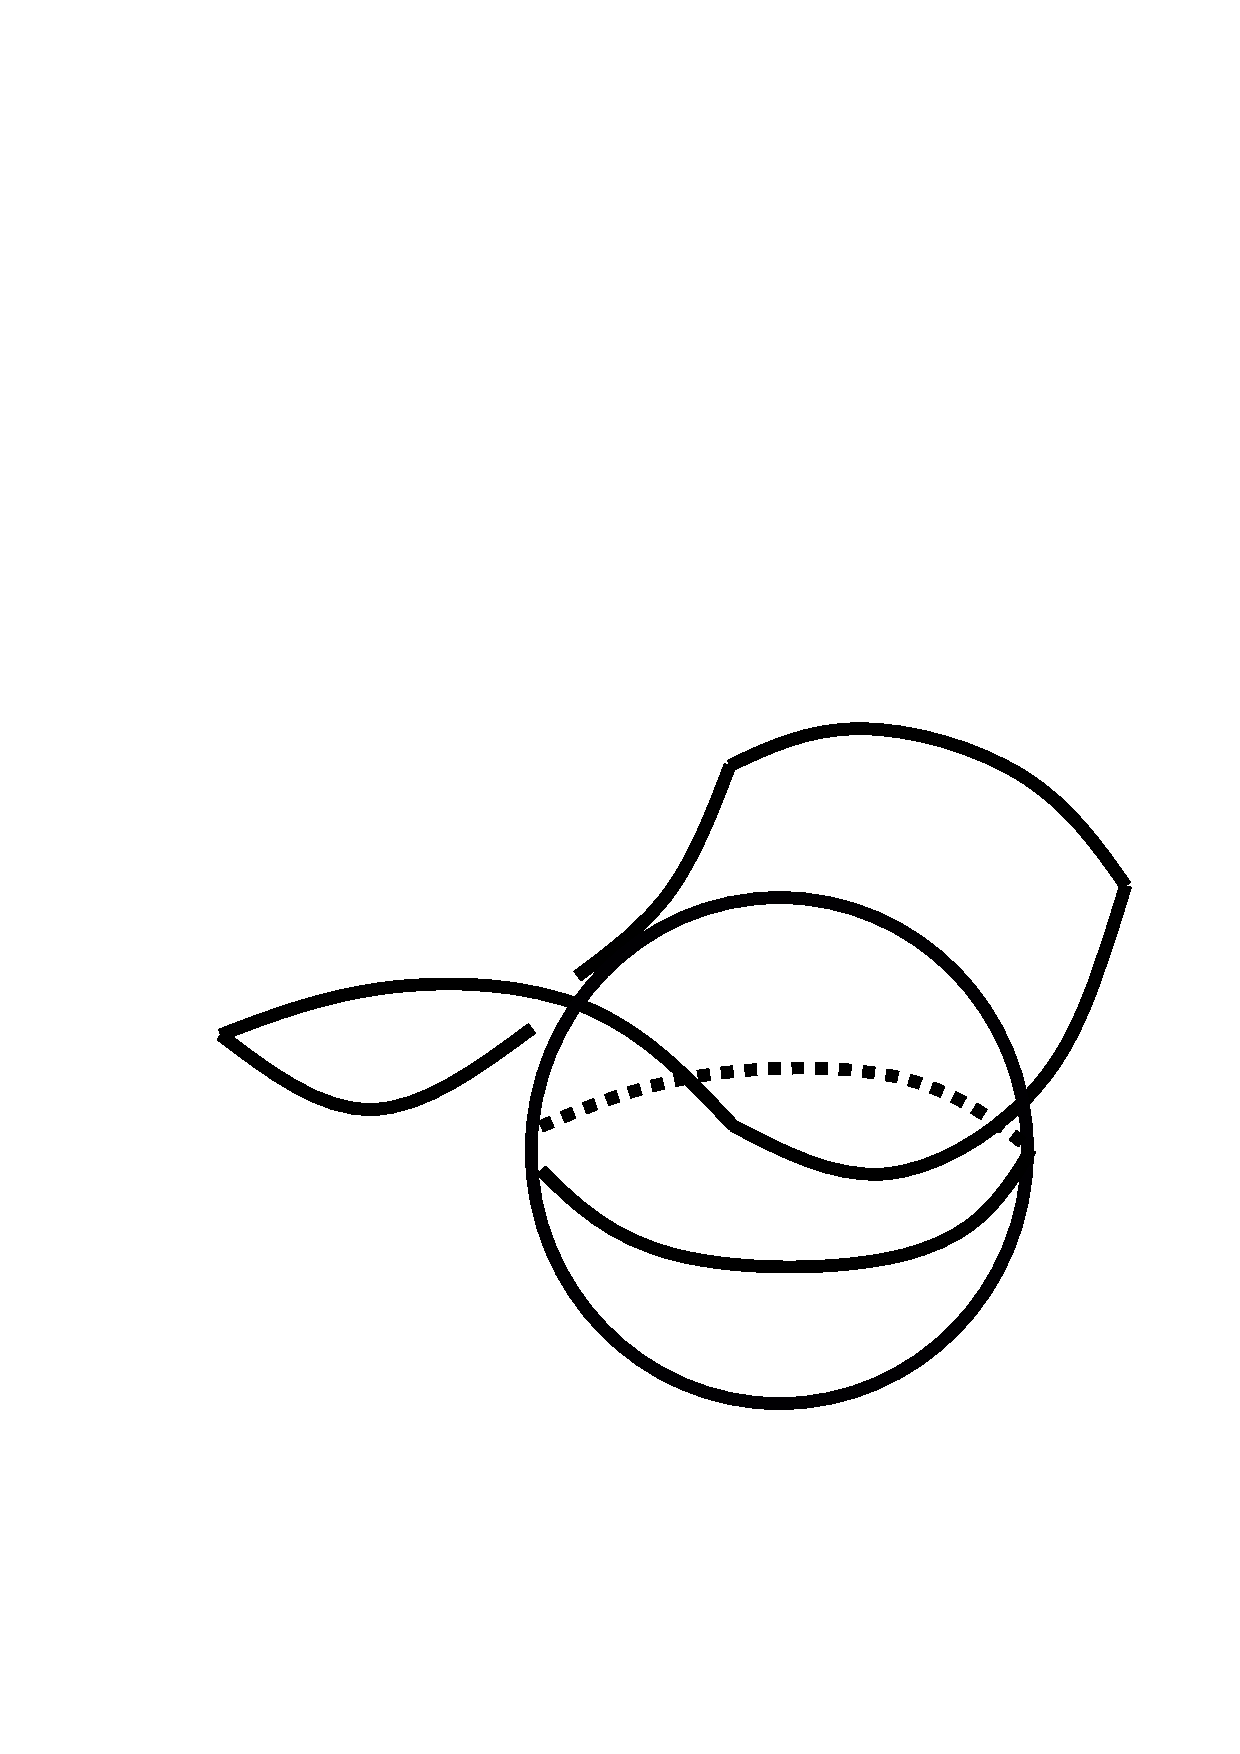
\includegraphics[width=\textwidth]{curvature/sphere-below-saddle}
        \subcaption{}\label{fig:sphere-below-saddle}
        \end{subfigure}
    \caption{(\subref{fig:sphere-above-saddle}) The osculating sphere above the saddle.
        (\subref{fig:sphere-below-saddle}) The osculating sphere above the saddle.
    }
    \label{fig:osculating-sphere}
\end{figure}


Since we assume that our surface $S$ is smooth, we have a well defined
tangent plane at the point of interest and a unit vector normal to the surface.
The \emph{Gauss map} is defined to be a map $g:S\rightarrow \Sp^2$
where, for $p\in S$ the value $g(p)$ is a unit vector orthogonal to $S$ at $p.$

The differential of the Gauss map, the \emph{Weingarten map}, is a linear 
transformation that maps the tangent
space of the surface at $p$ to the tangent space of the sphere at $N(p)$.
The determinate of the Weingarten map represents how the Gauss map
changes the area locally around $p$. 

Let $U_1$ be a `small' set on a convex surface $S$.
If the Gauss map is one-to-one on $U,$ and $g$ is orientation-preserving,
the curvature $K(U_1)$ of $U_1$ is defined to be the area of the image of $g(U_1)$
on $\Sp^2.$
Let $U_2$ be a nonconvex region on a surface on which $g$ is one-to-one and is orientation-reversing,
then $K(U_2)$ is defined as the negative of the area of $g(U_2)$ on $\Sp^2.$

\todo{Doesn't depend on area}

\begin{figure}[htb]
    \captionsetup[subfigure]{justification=centering}
    \centering
    \begin{subfigure}[b]{0.3\textwidth}
        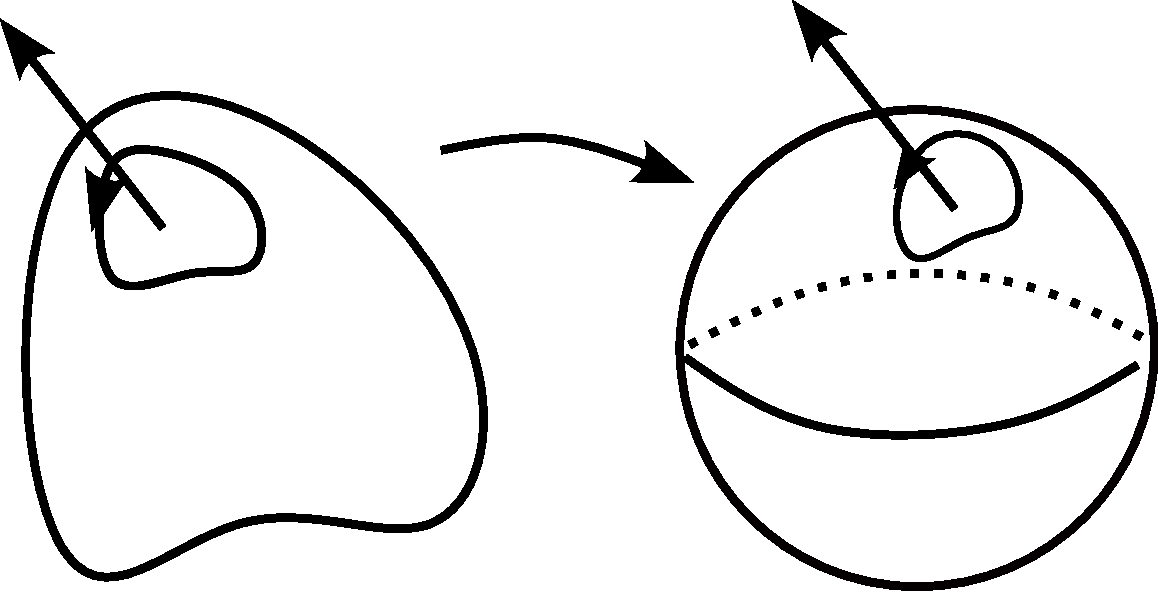
\includegraphics[width=\textwidth]{curvature/gauss-map-convex}
       \subcaption{}\label{fig:gauss-map-convex}
    \end{subfigure}
        \hspace{1cm}
        \begin{subfigure}[b]{0.3\textwidth}
        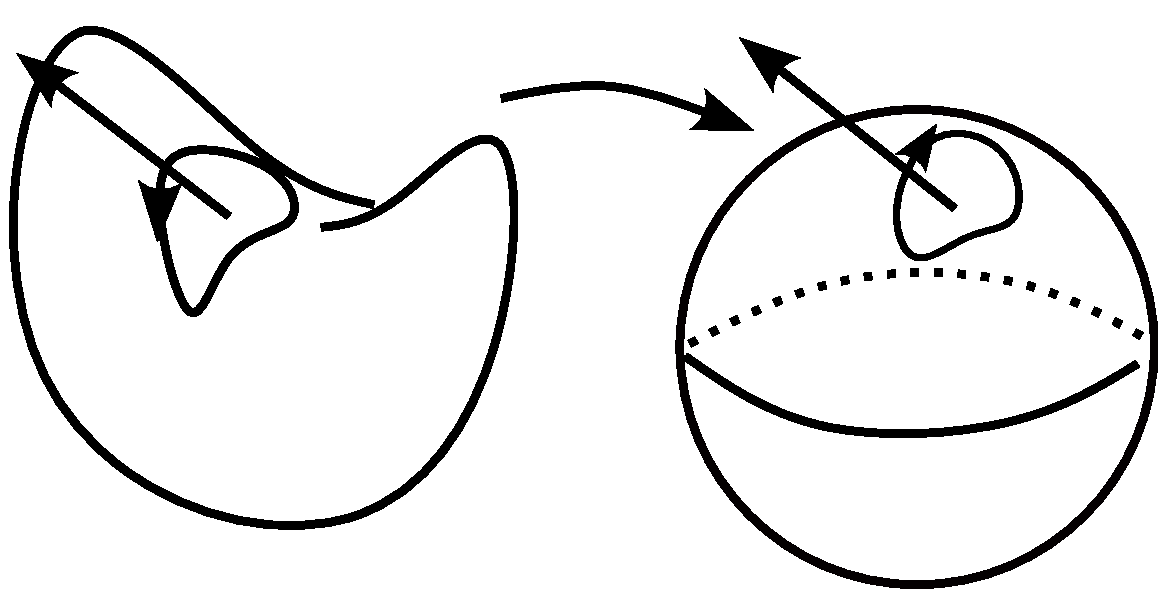
\includegraphics[width=\textwidth]{curvature/gauss-map-nonconvex}
        \subcaption{}\label{fig:gauss-map-nonconvex}
        \end{subfigure}
    \caption{(\subref{fig:gauss-map-convex}) The Gauss map on a convex region.
        (\subref{fig:gauss-map-nonconvex}) The Gauss map on a nonconvex region.
    }
    \label{fig:normal-sections}
\end{figure}

Here is an another definition of curvature.
Every plane containing the normal vector will intersect the surface.
The intersection of the surface and each normal plane is a curve in $\RR^3$
gives a one dimensional curve called the \EMPH{normal section}, see  \figref{normal-sections}
for an example.
Let $\kappa_1$ denote the maximum curvature of all normal sections 
and let $\kappa_2$ denote the minimum. 
The \EMPH{Gaussian curvature} of a point on a surface is
$K=\kappa_1\kappa_2.$
One can check that the Gaussian curvature of the plane is zero and
that larger circles have less curvature than smaller ones.



\begin{figure}[htb]
    \captionsetup[subfigure]{justification=centering}
    \centering
    \begin{subfigure}[b]{0.25\textwidth}
        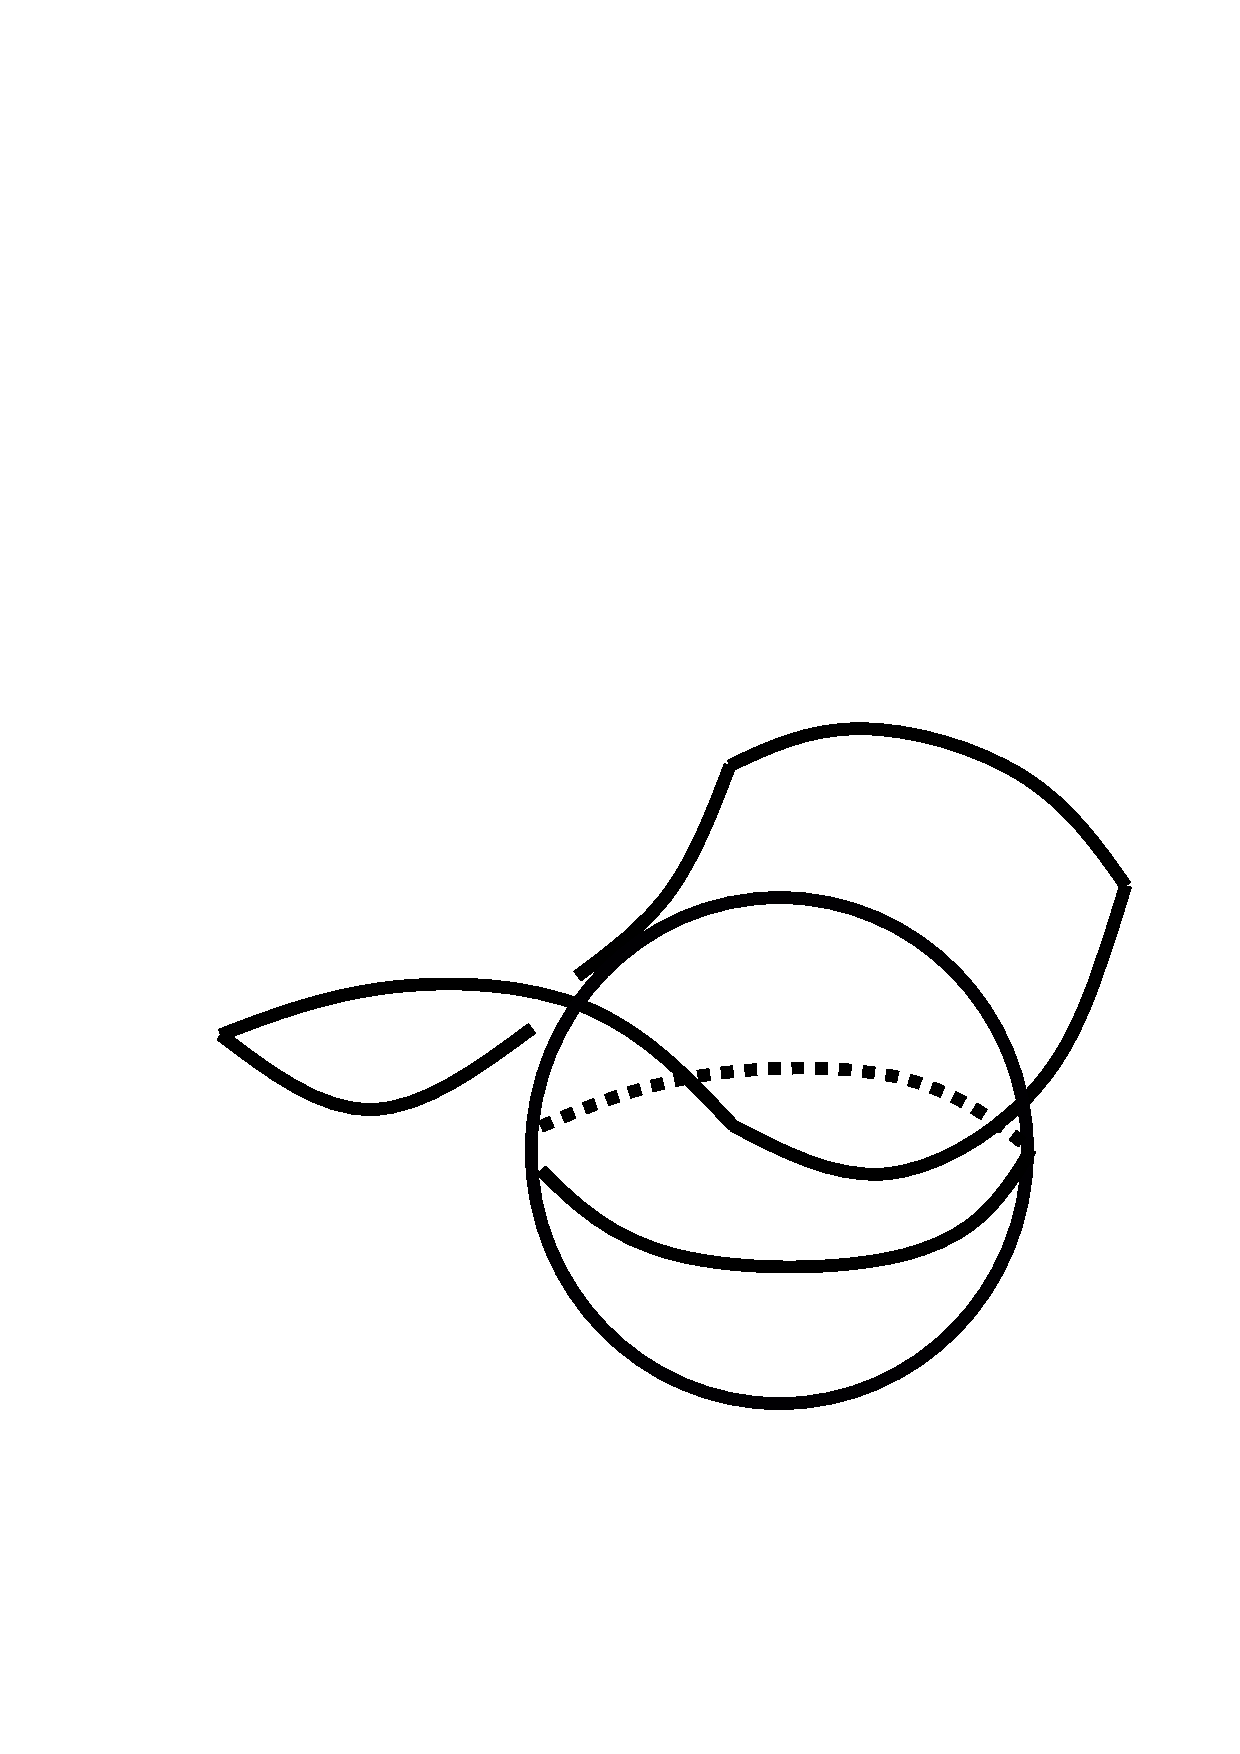
\includegraphics[width=\textwidth]{curvature/normal-section-max}
       \subcaption{}\label{fig:normal-section-max}
    \end{subfigure}
        \hspace{1cm}
        \begin{subfigure}[b]{0.25\textwidth}
        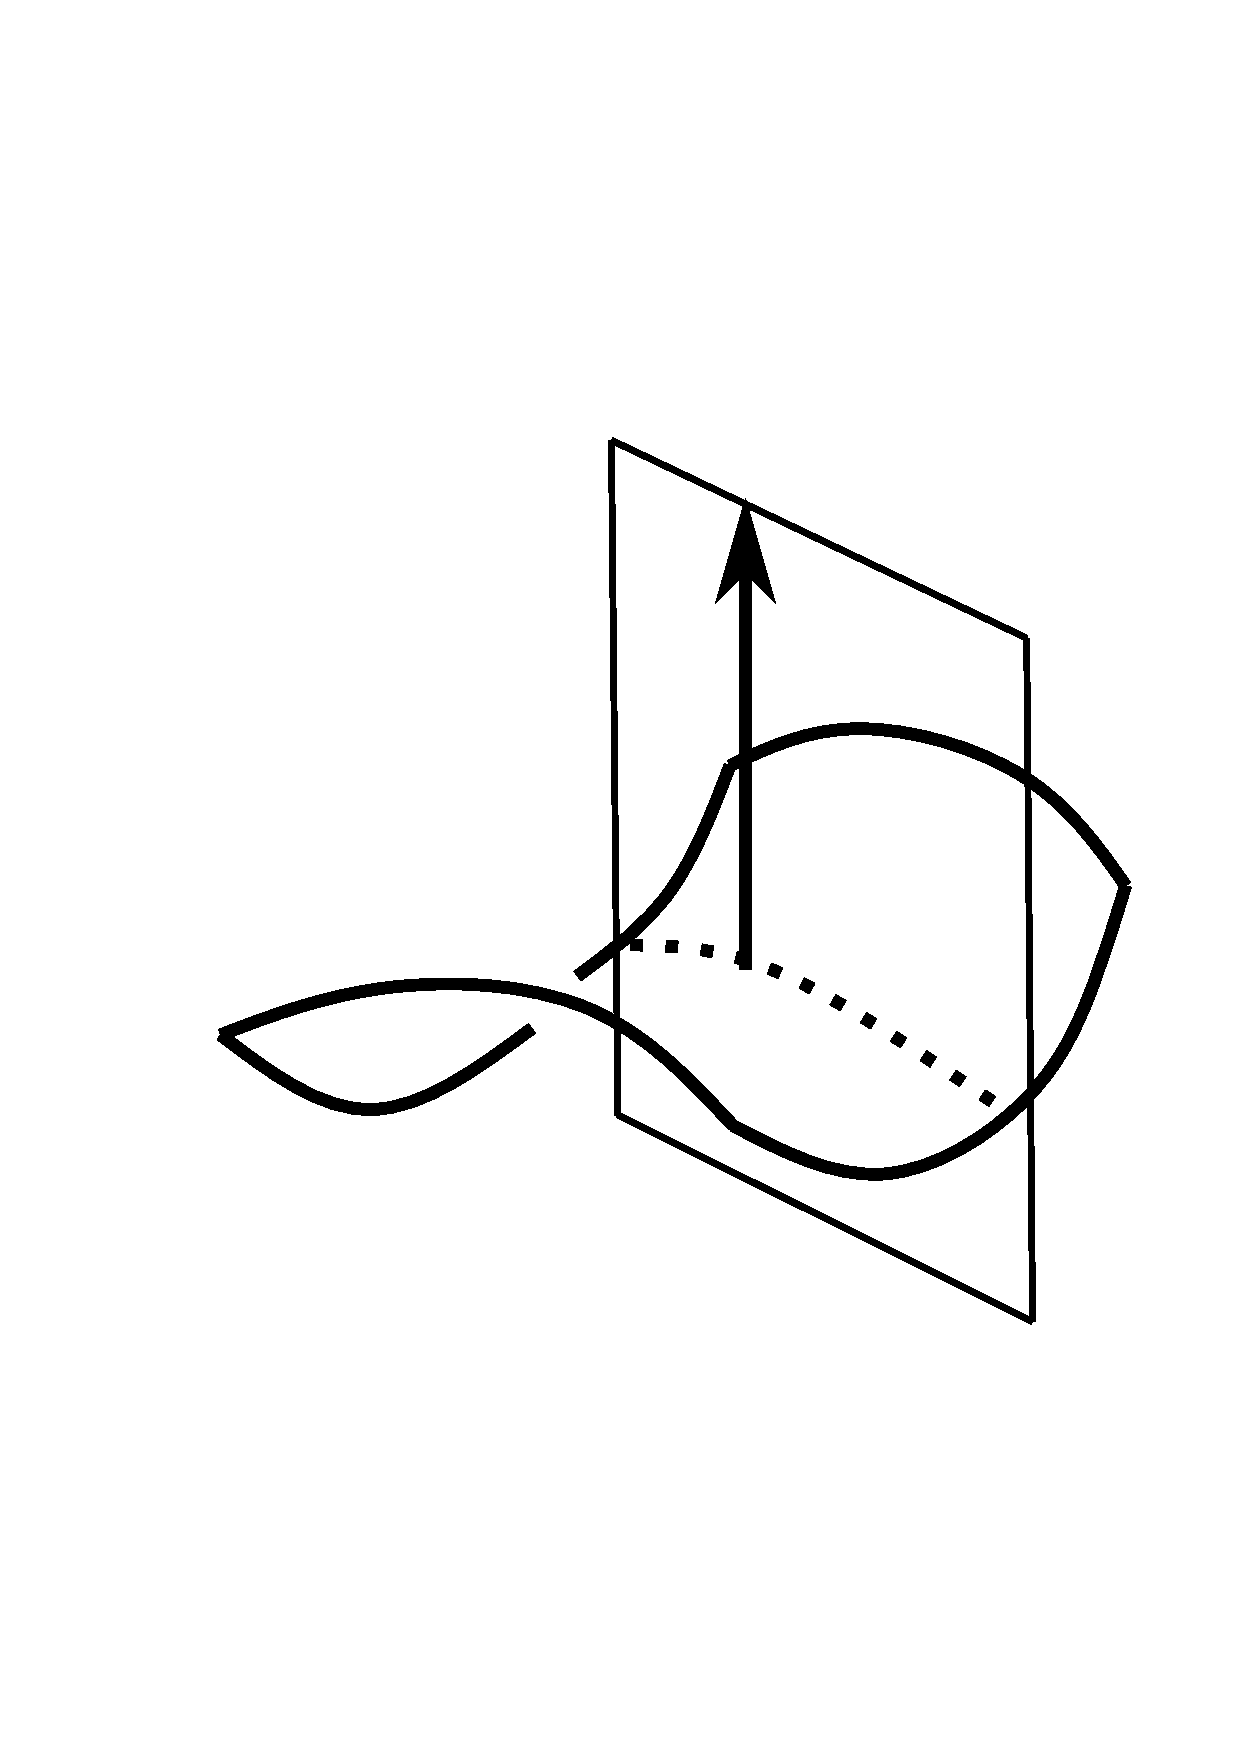
\includegraphics[width=\textwidth]{curvature/normal-section-min}
        \subcaption{}\label{fig:normal-section-min}
        \end{subfigure}
    \caption{(\subref{fig:normal-section-max}) The osculating sphere above the saddle.
        (\subref{fig:normal-section-min}) The osculating sphere above the saddle.
    }
    \label{fig:normal-sections}
\end{figure}


\subsection{Computing Curvature}
We now consider computing the Gaussian curvature.
A \EMPH{quadratic form} to be polynomial of degree two, of the form $p(u,v)=c_1u^2+c_2uv+c_3v^2$ 
where $c_i\in R$.
We define a quadratic form, the first fundamental form, using $r(u,v)$.

Let $r(u,v)$ be a parameterized surface.
Let $E=r_u\cdot r_u, F=r_u\cdot r_v$ and  $G=r_v\cdot r_v$.
The \EMPH{first fundamental form}
is the quadratic form $\mathrm{I}=Edu^2+2Fdudv +Gdv^2$.
We summarize the first fundamental form as a matrix $$\mathrm{I}=\begin{bmatrix}
E & F \\
F & G 
\end{bmatrix}.$$
%We get a notion of length in the tangent space, an inner product on $Tp(S)$.
%If $x$ and $y$ are two tangent vectors
%then $$\mathrm{I}(x,y)=x^T\begin{bmatrix}
%E & F \\
%F & G 
%\end{bmatrix}y.$$

The first fundamental form enables us to  compute many interesting
things about our surface including arc length, angles between curves,
and area on a surface.
For example,
given a `small' parallelogram $M$ on $S$ with corners $r(u,v),r(u+\epsilon u, v), r(u,v+\epsilon v)$ 
and $r(u+\epsilon u, v+\epsilon v)$ the rate of change of the area of $M$ is 
$$dA=\sqrt{EG-F^2}dudv.$$
In \exref{stereo}, we will use the first fundamental form to compute the arc length of some curves.


Gauss's Egregious (remarkable) Theorem states that the Gaussian curvature only depends
of the first fundamental form. Thus, curvature can be computed entirely by measuring angles, distance 
and their derivatives without any reference to the way that the surface is embedded in $\R^3.$
Because of this property we say that Gaussian curvature is an \emph{intrinsic} property of a surface.
The Brioschi formula gives the Gaussian curvature using only the first fundamental form
\begin{equation}\label{eq:brioschi}
	K=\frac{\begin{vmatrix}
-\frac{1}{2}E_{vv}+F_{uv}-\frac{1}{2}G_{uu} & \frac{1}{2}E_u & F_u-\frac{1}{2}E_v\\
F_v-\frac{1}{2}G_u & E & F\\
\frac{1}{2}G_v & F & G
\end{vmatrix}-\begin{vmatrix}
0 & \frac{1}{2}E_v & \frac{1}{2}G_u\\
\frac{1}{2}E_v & E & F\\
\frac{1}{2}G_u & F & G
\end{vmatrix}}{(EG-F^2)^2}
\end{equation}



While we can compute Gaussian curvature using only the first fundamental form,
 the second fundamental form is convenient for computations.
To this end, the unit normal vector at $p$ is given by $$n(p)=\frac{r_u\times r_v}{|r_u\times r_v|}.$$
Let $L=r_{uu}\cdot n, M=r_{uv}\cdot n$ and $N=r_{vv}\cdot n$ the
\EMPH{second fundamental form} is $\mathrm{I\!I}=Ldu^2+2Mdudv+Ndv^2$,
in matrix form $$\mathrm{I\!I}=\begin{bmatrix}
L & M \\
M & N 
\end{bmatrix}.$$
%Another inner product is given by $$\mathrm{I\!I}(x,y)=x^T\begin{bmatrix}
%L & M \\
%M & N 
%\end{bmatrix}y.$$
Combining the first and second fundamental forms we have
the \EMPH{Gaussian curvature} of a surface is
\begin{equation}\label{eqn:curve-dets}
 	K=\frac{\det(\mathrm{I\!I})}{\det(\mathrm{I})}.
\end{equation}

\begin{example}[Curvature of the Sphere]\label{ex:compute-surface-curvature}
Consider the northern hemisphere of the unit sphere parameterized
by $$r(u,v)=(u,v,\sqrt{1-u^2-v^2})$$ and we wish to compute the Gaussian curvature at
the north pole $p=(0,0,1)$.
We have $$r_u|_p=(1,0,\frac{-u}{\sqrt{1-u^2-v^2}})|_p=(1,0,0)$$ and
$$r_v|_p=(0,1,\frac{-v}{\sqrt{1-u^2-v^2}})|_p=(0,1,0).$$
We have $E=1, F=0,$ and $G=1$ so our first fundamental form is
$\mathrm{I}=\begin{bmatrix}
1 & 0 \\
0 & 1 
\end{bmatrix}.$
Our normal vector is $n(p)=(0,0,1)$ with 
$$r_{uu}|_p=(0,0,\frac{1-2u^2}{(1-u^2)^{\frac{3}{2}})})|_p=(0,0,1),
r_{uv}|_p=(0,0,0)$$ and 
$$r_{vv}|_p=(0,0,\frac{1-2v^2}{(1-v^2)^{\frac{3}{2}})})|_p=(0,0,1).$$
Thus, $L=1, M=0$ and $N=1$ and our second fundamental form is
$\mathrm{I\!I}=\begin{bmatrix}
1 & 0 \\
0 & 1 
\end{bmatrix}$
and our Gaussian curvature is $K=\frac{\det(\mathrm{I\!I})}{\det(\mathrm{I})}=\frac{1}{1}=1$ as expected.

\end{example}

We will use the first fundamental form to compute
the arc length of circles on the sphere parallel to the $xy$ plane with fixed height $z=c$ for $-1<c<1$.
Stereographic projection, described in \secref{plane-sphere},
allows us map our problem to the plane and perform our computations there.

\begin{example}[Stereographic Projection Revisited\cite{christian-notes}]\label{ex:stereo}
Consider the two sphere with the north pole removed $\Sp^2 \setminus (0,0,1)$,
stereographic projection is a bijection between the points on $\Sp^2 \setminus (0,0,1)$ to the $\R^2$.
Consider a line from the north pole $(0,0,1)$ that intersects $(x,y,z)\in \Sp^2$ parametrized by 
$p(t)=(1-t)(0,0,1)+t(x,y,z)$. By considering the $z$ coordinate we determine the $t$ value where this line
intersects $\R^2$, namely $t=\frac{1}{1-z}.$
This gives the desired map shown in \figref{stereo} and in equation form
$$p(x,y,z)\to \left(\frac{x}{1-z},\frac{y}{1-z}\right).$$

\begin{figure}[htb]
	\centering
	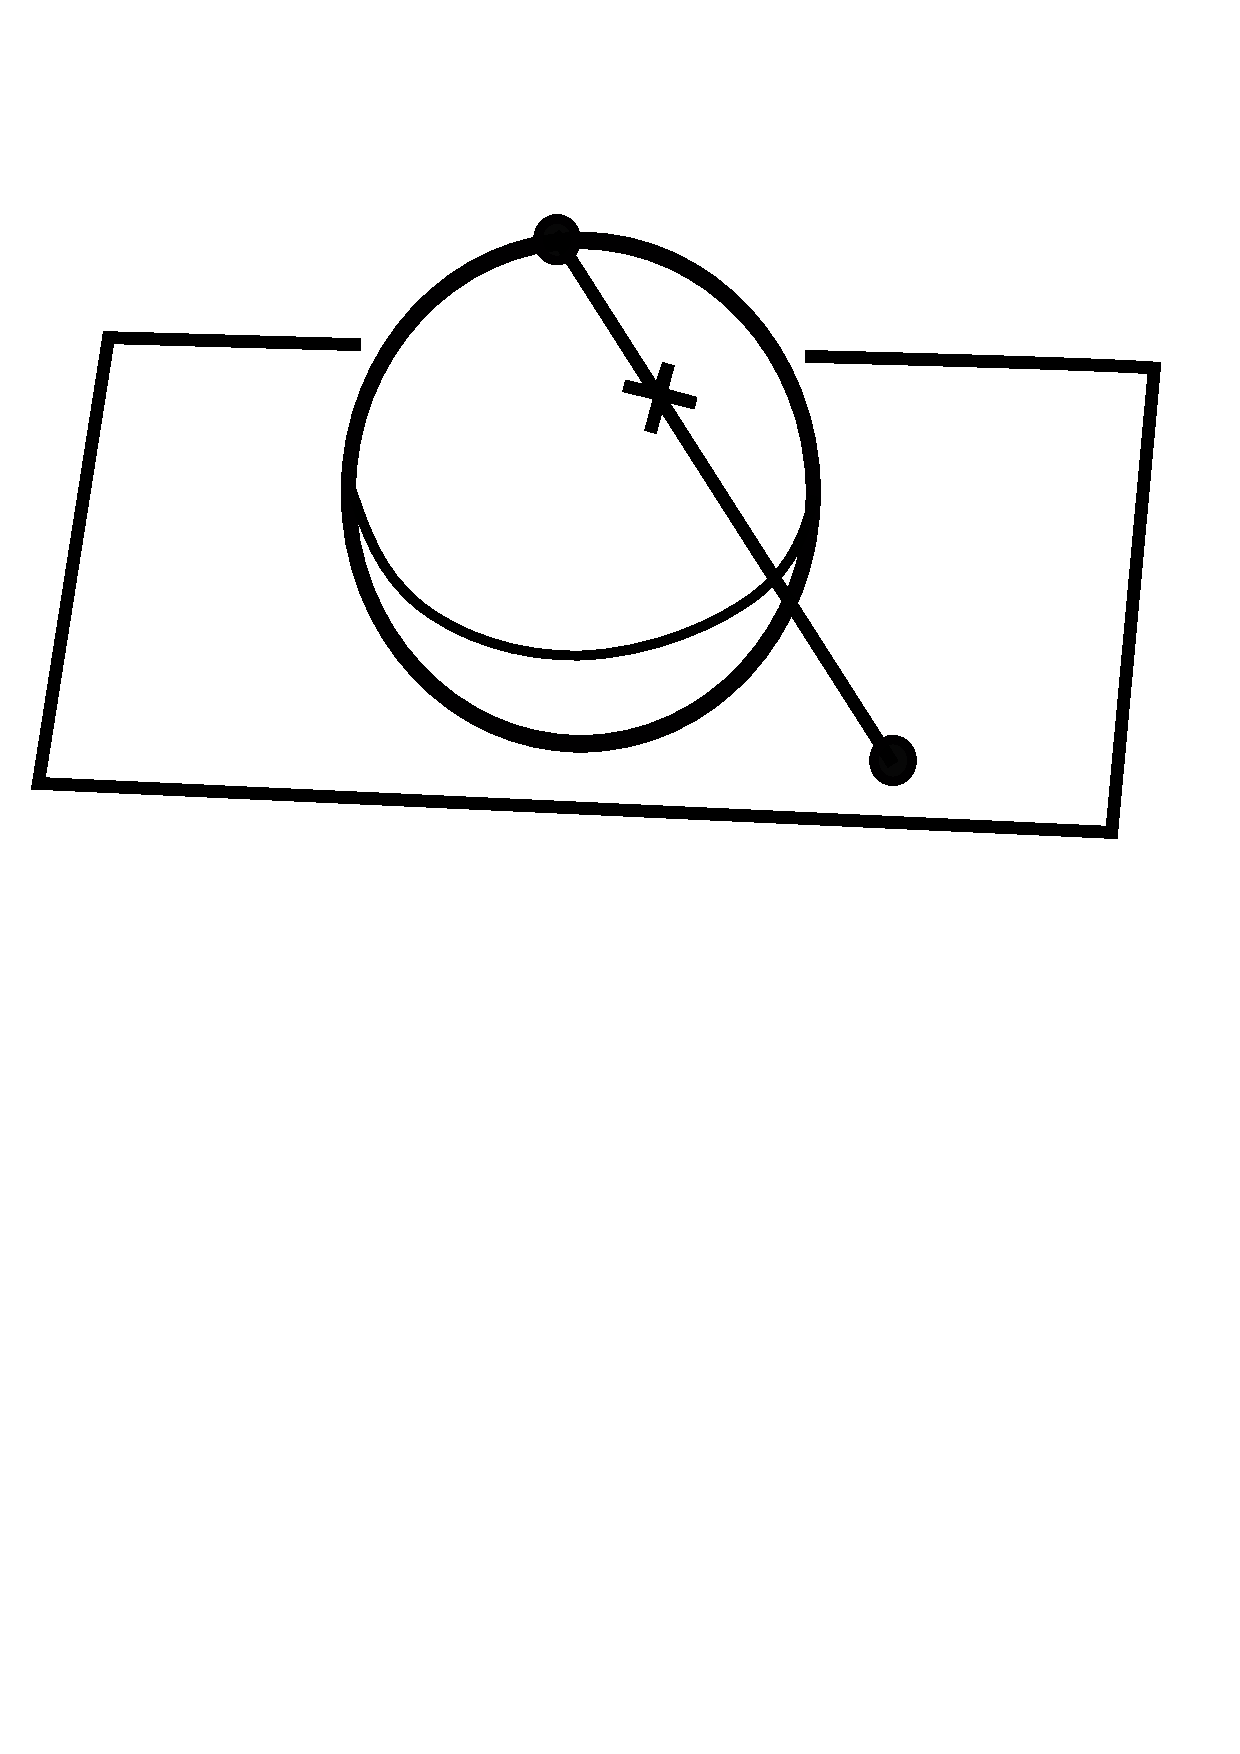
\includegraphics[width=.3\textwidth]{curvature/stereo}
	\caption{A point on the sphere is mapped to a point on the plane by stereographic projection.}
	\label{fig:stereo}
\end{figure}
	
The inverse is given by $p^{-1}:\R^2\to \R^3$

	\begin{equation}\label{eqn:stereo}
		p^{-1}(u,v)=\left(\frac{2u}{u^2+v^2+1},\frac{2v}{u^2+v^2+1},\frac{u^2+v^2-1}{u^2+v^2+1}\right).	
	\end{equation}
To compute the first fundamental form of $p^{-1}(u,v)$ we take the partial derivatives

$$p^{-1}_u=\left(\frac{2v^2-2u^2+2}{(u^2+v^2+1)^2},\frac{-4uv}{(u^2+v^2+1)^2},\frac{4v}{(u^2+v^2+1)^2}\right)$$
and 
$$p^{-1}_v=\left(\frac{-4uv}{(u^2+v^2+1)^2},\frac{2v^2-2u^2+2}{(u^2+v^2+1)^2},\frac{4v}{(u^2+v^2+1)^2}\right).$$
Then, after some algebra,
$$E=p^{-1}_u\cdot p^{-1}_u=\frac{4}{(u^2+v^2+1)^2}$$
$$F=p^{-1}_v\cdot p^{-1}_v=\frac{4}{(u^2+v^2+1)^2}$$
and
$$M=p^{-1}_u\cdot p^{-1}_v=0.$$

We can use the first fundamental form to compute
the arc length of circles on the sphere parallel to the $xy$ plane with fixed height $z=c$ for $-1<c<1$.
This length can be computed using
the pythagorean theorem. We will see that using stereographic projection
and the first fundamental form we get the same answer.


The arc length of a parameterized curve $u=u(t), v=v(t)$ on a regular surface,
can be computed using the first fundamental form.  Let
$s$ denote the arc length, then 
$$ds=\bigg | \frac{dr}{dt}\bigg | dt = \bigg | r_u\frac{du}{dt}+r_v\frac{dv}{dt}\bigg |dt
=\sqrt{(r_u^2 du^2+2r_ur_v du dv + r_v^2dv^2)}.$$
Next, use the map $p$ to map such a circle to the plane.
Using \eqnref{stereo}, our circle on the sphere maps 
to a circle in the plane because
	$$p^{-1}(u,v)=\frac{u^2+v^2-1}{u^2+v^2+1}=c$$
and we can compute the radius in terms of $c$
\begin{equation}\label{eqn:radius}
	u^2+v^2=\frac{1+c}{1-c}=k^2.
\end{equation}
	
In the plane, $u^2+v^2=k^2$ can be parameterized
as $$\gamma(t)=(k\cos(t),k\sin(t))$$ with $0\leq t\leq 2\pi.$
So our curve becomes $p^{-1}\circ \gamma(t)$ on the sphere.
Computing the partial derivatives of $\gamma(t)$ gives
$$\gamma_u'=-k\sin(t)\hspace{1.3cm}  \gamma_v'=k\cos(t).$$
Now we use the first fundamental form

$$\int_{p^{-1}}\gamma ds=\int_{0}^{2\pi} ||(p^{-1}\circ \gamma)'(t)dt=\int_0^{2\pi}\sqrt{E(\gamma_u'(t))^2+2M\gamma_u'\gamma_v'+
F(\gamma_v'(t))^2}dt.$$
Substituting and simplifying using $E=F$ we obtain
$$\int_0^{2\pi}\frac{2k}{k^2+1}dt=\frac{4\pi k}{k^2+1}.$$
Simplifying further using \eqnref{radius}  our arc length is
$$2\pi\sqrt{1-c^2}.$$

\end{example}



\begin{theorem}[First Fundamental Form and Conformal Maps]\label{thm:first-conformal}
	Let $S$ be a regular surface and $f:U\subset \R^2 \to V\subset S$ be a chart.
	Let $f$ have first fundamental form $\mathrm{I}=Edu^2+2Fdudv +Gdv^2$.
	Then $f$ is conformal if and only if $E=G$ and $F=0.$
\end{theorem}

\subsection{Discrete Gaussian Curvature}
\label{sec:discrete}


We use a discrete version of the Guass map to define curvature
of a vertex of a polygonal surface.
Recall, that when we considered the curvature at a vertex on a polygon in the plane
in the theorem of turning tangents, \thmref{simple-bonnet}, we have two equivalent
formulations depending on
weather we use the interior or the exterior angles at each vertex.
We can do a similar thing with the discrete Gaussian curvature at a vertex on a surface,
instead of considering the angles of the faces incident to a vertex $v$, we can consider
the complementary angle. The complementary angle is shown in \figref{switcheroo}. 
If we let $n$ be the number of faces
incident to $v$, the formula for the discrete curvature then becomes
\begin{equation}\label{eqn:discrete-curvature-complement-angle}
K(v)=2\pi - \sum_{i=1}^n (\pi - \xi_i)=(2-n)\pi +\sum_{i=1}^n \xi_i.
\end{equation}
By \eqnref{sphere-area}, this is the area of the polygon on the sphere with interior
angles $\xi_1, \xi_2,\ldots \xi_n.$
Geometrically, this angle be seen in \figref{switcheroo}.
If we project the normal vectors on each face onto a sphere and
connect these points with great arcs to create a polygon on the sphere with interior angles
$\xi_1, \xi_2,\ldots \xi_n.$
We have a geometric representation of discrete
Gaussian curvature as the area on the unit 
sphere bounded by a spherical polygon whose vertices are the unit normals of 
the faces around $v$. An example is shown in \figref{discrete-curvature}.

\begin{figure}[htb]
\centering
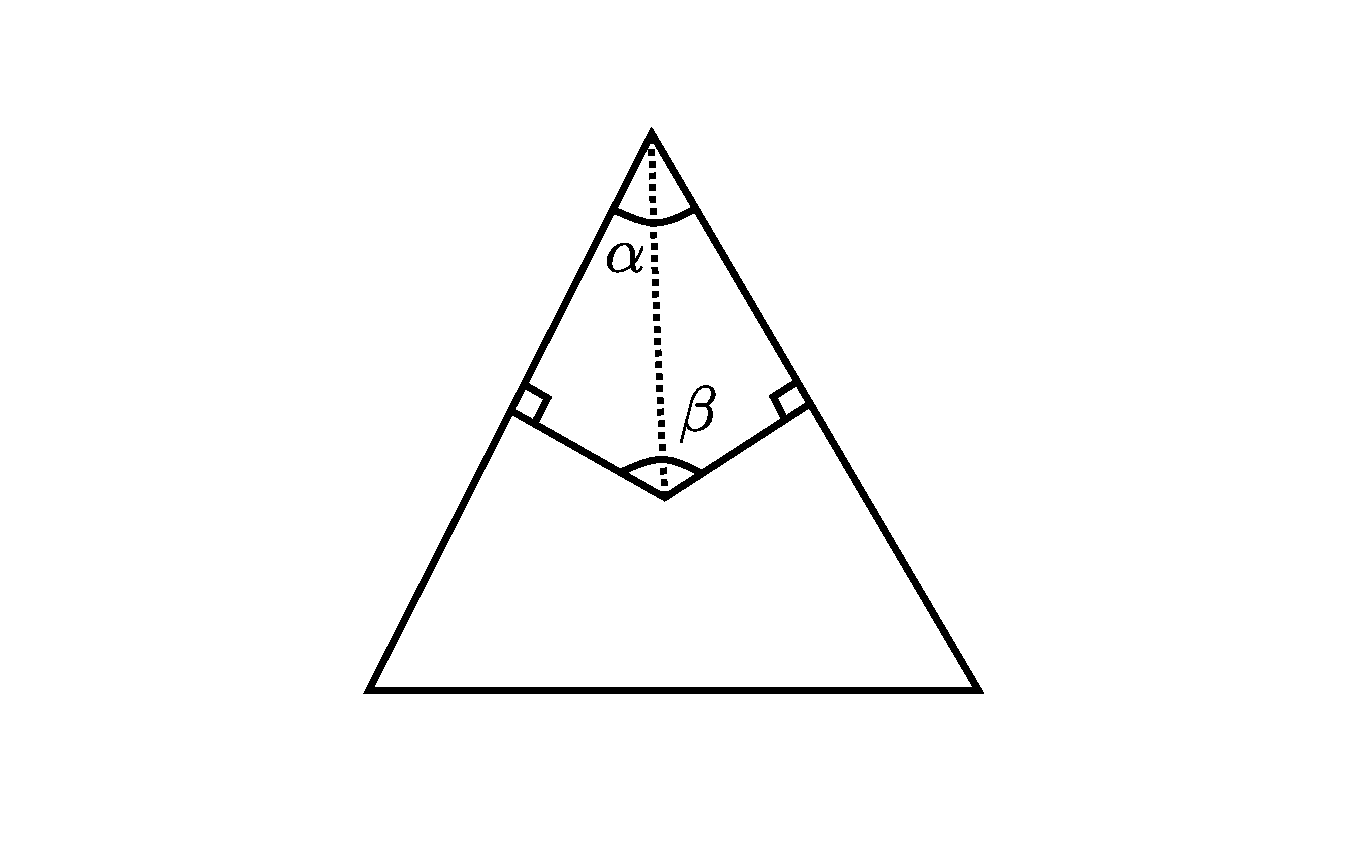
\includegraphics[width=.25\textwidth]{background/switch-angles}
\caption{The relationship between the angles incident to a vertex and
its complementary angle.}
\label{fig:switcheroo}
\end{figure}





\begin{figure}[htb]
\centering
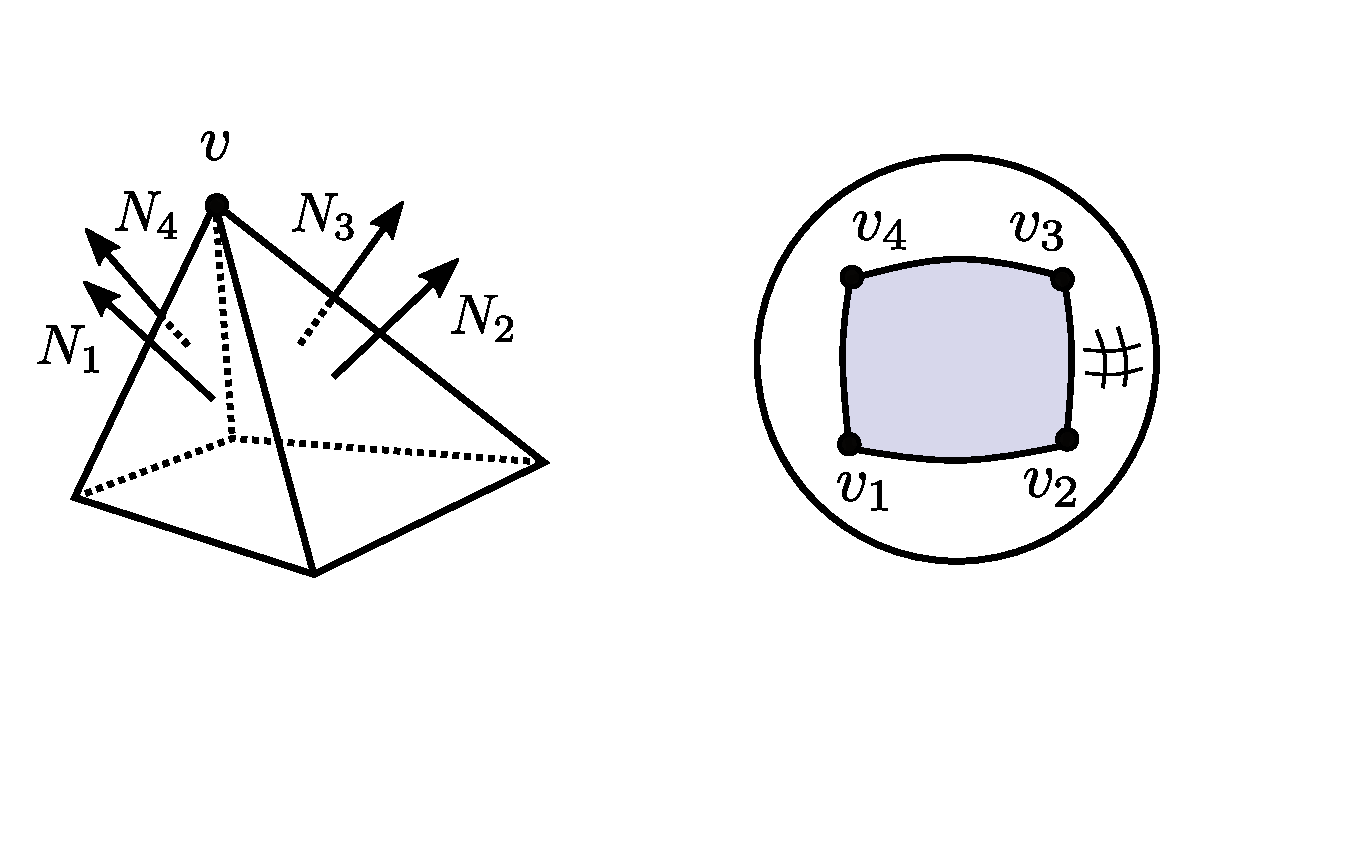
\includegraphics[width=.5\textwidth]{curvature/discrete-curvature}
\caption{Consider the vertex $v$ in the figure on the left. The curvature of $v$
is the area on the sphere shown on the right. We rotated the sphere
in order to see the entire polygon.}
\label{fig:discrete-curvature}
\end{figure}







We can use a continuous version of the Gauss-Bonnet theorem to derive
the same expression for discrete curvature at a vertex on a polygonal surface,
which we now describe.
Note that we need to be cause full not to use the Gauss-Bonnet theorem to
define curvature then use curvature to prove the theorem. 
We already have a definition of discrete curvature above. We include this derivation
as an application of the continuous Gauss-Bonnet theorem.

Recall, in one dimension, we defined the discrete curvature of a vertex in a
polygonal curve to be exterior angle.
Consider a triangulated polygonal surface $T$ with boundary $\partial(T)$.
The boundary is a one dimensional piecewise linear curve in $\R^3.$
As with polygons in the plane, at each vertex $v\in \partial(T)$ 
we have an exterior angle.

The interior angle might consist of many triangles.
Let $F_v$  denote the set of faces incident to $v$ and let
$\alpha_f$ denote the angle in face $f$ at $v$.
The \EMPH{discrete geodesic curvature}
of $v$  is
$$k_{g}(v)= \pi-\sum_{f\in F_v}\epsilon_f.$$
See \figref{discrete-geodesic} for an illustration.
Notice that if $v$ lies on a straight line, then $\sum_{i}\epsilon_f=\pi$
and the curvature is zero as we would expect.


\begin{figure}[htb]
\centering
	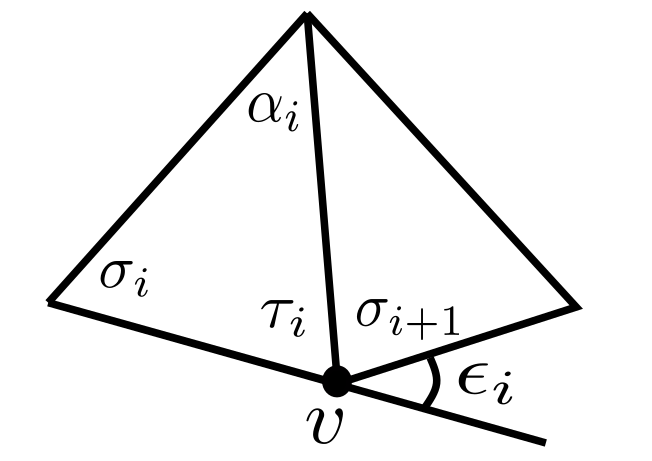
\includegraphics[width=.25\textwidth]{curvature/discrete-geodesic}
	\caption{The discrete geodesic curvature at a vertex $v$ on the boundary
	of a surface is given by the exterior angle $\epsilon$.}
	\label{fig:discrete-geodesic}
\end{figure}


At every non-vertex point on a polygonal surface, the continuous Gaussian curvature
is zero and at every vertex it is undefined.
We can use the intuitive definition of discrete geodesic curvature and the Gauss-Bonnet
theorem to give a definition for discrete Gaussian curvature.

Consider removing the neighborhood around a vertex $v$ consisting
of the faces incident to $v$ and the edges and vertices of these faces call
this $N(v)$.
Using the variable names given in \figref{discrete-geodesic},
the total geodesic curvature

\begin{align}
\int_{\partial N(v)} kg ds &=\sum_i \pi -(\tau_i+\sigma_{i+1})\nonumber  \\
       &=\sum_i \pi -(\tau_i+\sigma_{I}) \nonumber  \\
       &=\sum_i \alpha_i. \nonumber 
\end{align}
Where the second equality comes from the boundary being a circle and reorganizing the sum.
Topologically, this neighborhood is a disk and $\chi(N(v))=1$
so the Gauss-Bonnet theorem tells us that 
the discrete Gaussian curvature at a vertex is
\begin{definition}[Discrete Gaussian curvature\footnote{Discrete Gaussian curvature
is also called the \emph{angle defect} at a vertex}]\label{def:discrete-curvature-vertex}

$$K(v)=\int_{N(v)}K da=2\pi-\sum_i \alpha_i.$$

\end{definition}

\subsection{Reducing the Size of a Mesh}
\label{sec:removing}

The definition of discrete Gaussian curvature that we
derived by applying the Gauss-Bonnet theorem is used when 
a triangulated surface is generated by scanning an object.
In this context, a triangulated surface is called a mesh.

Meshes that are obtained by scanning real objects contain noise.
Most meshes that are generated by scanning require a complete
remeshing \cite{remeshing-2003}.
As a first step in remeshing, the curvature at each
vertex needs to be estimated \cite{mmsb-2003}.




Computing the curvature at each vertex in a mesh can allow one to reduce
the number of vertices in the mesh without sacrificing mesh quality.
This leads to simplification process that reduces storage space and improves the efficiency of
 algorithms run on the mesh.
If the curvature at a vertex is zero, then the vertex can be removed,
along with the faces and edges incident to the vertex, without changing 
the mesh.
 If the curvature is small, then few points
are sampled to be included in the re-mesh. If the curvature
is large, then many points are sampled. See \figref{planck-mesh}
for an illustration.

\begin{figure}[htb]
\centering
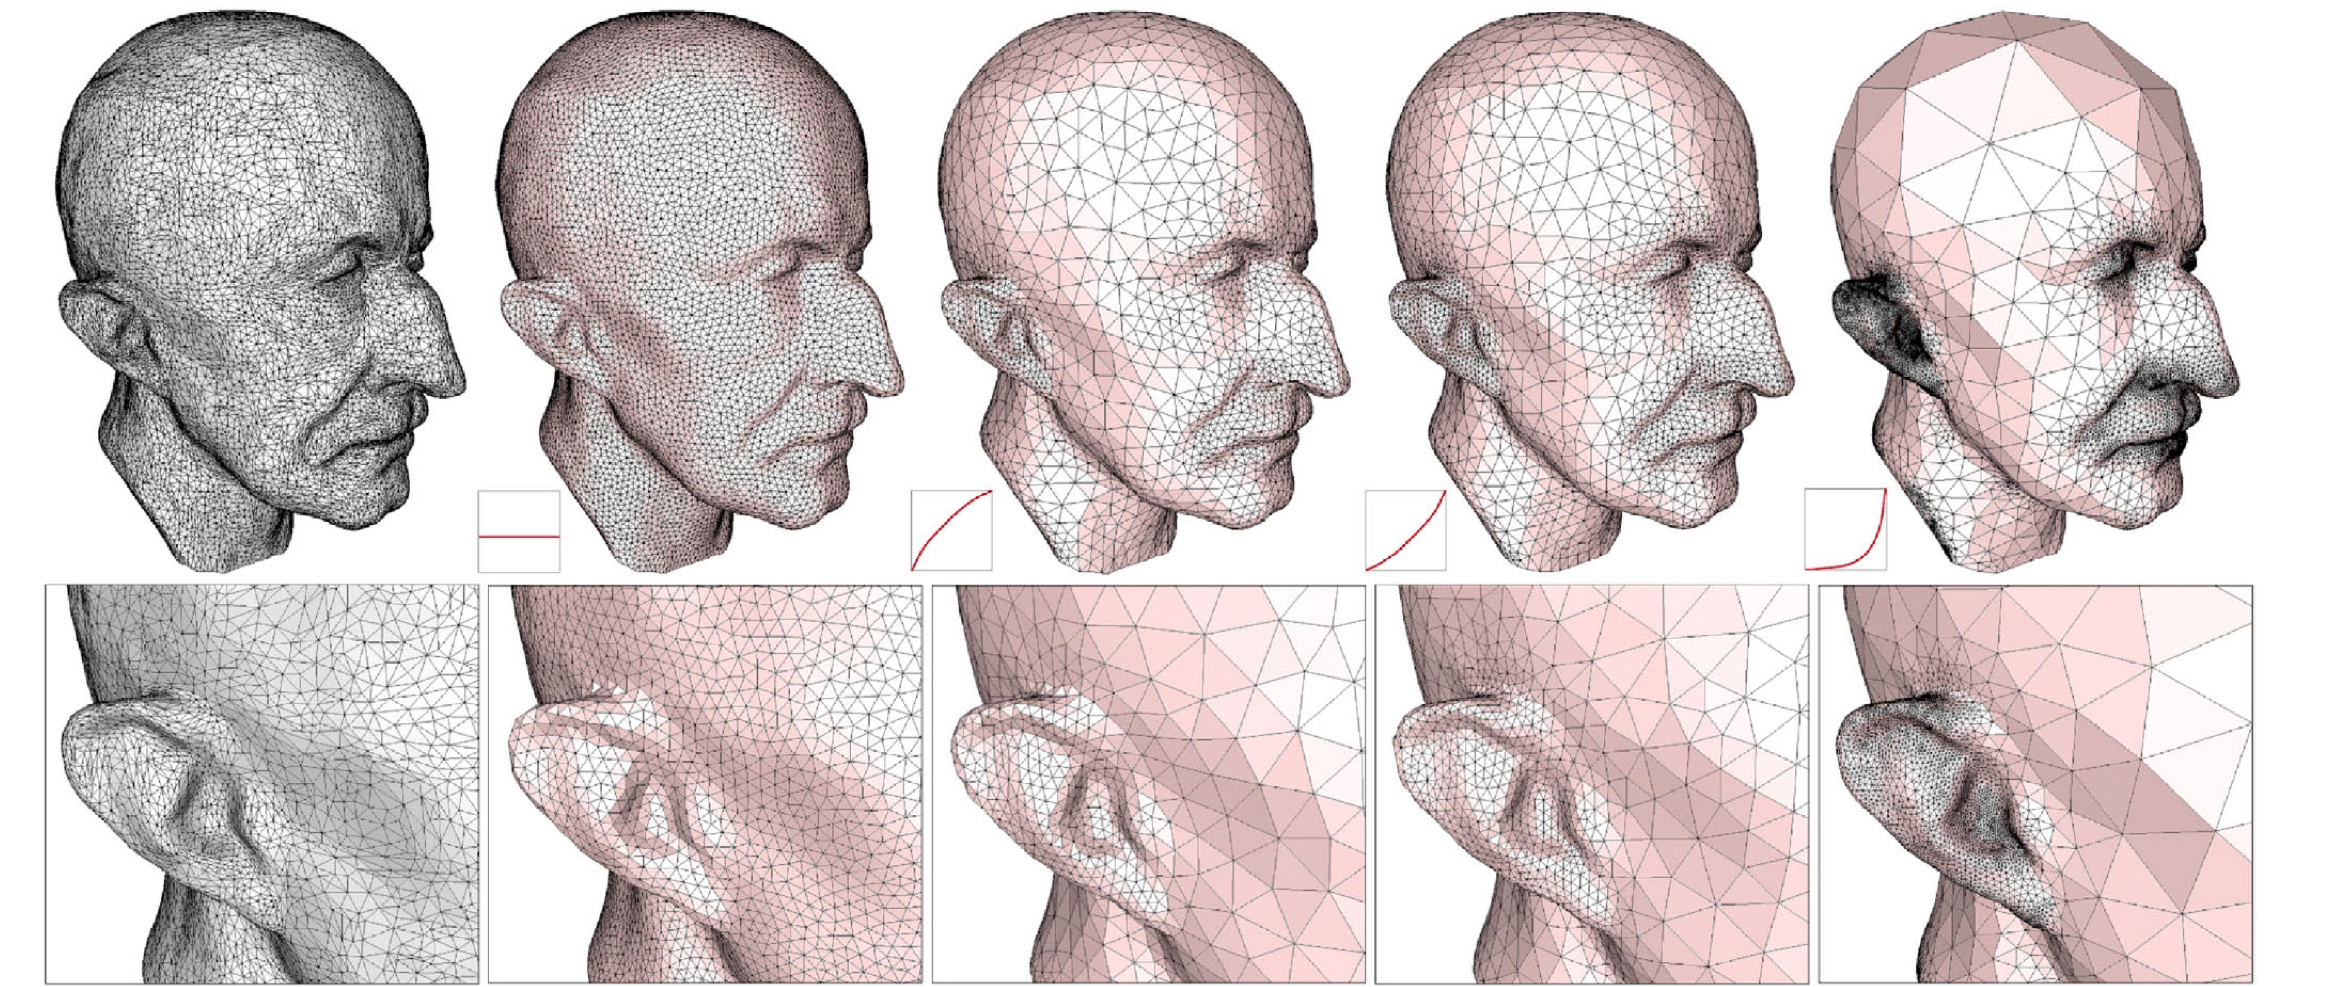
\includegraphics[width=.7\textwidth]{meshes/planck-mesh.jpeg}
\caption{A mesh of Max Plank. The original mesh is on the left. As we move
from left to right more importance is placed on vertices with large curvature.
Figure from \cite{alliez-2002}.}
\label{fig:planck-mesh}
\end{figure}


The experiments in \cite{mmsb-2003} found that the average
percent error did not exceed $1.3\%$ when using this operator.\todo{what does
this mean?}



\subsection{Geodesics Curvature}

Shortest paths play an important role in many computational problems.
On a surface, a \EMPH{geodesic} is a curve that is a shortest path
between two points in the surface. 
For example, on $\Sp^2$ great circles are geodesic.
Intuitively, the geodesic curvature of a one dimensional curve on a surface
is the curvature as it would be seen from someone living on the surface.


Given a parameterized surface and a point on parameterized curve on the surface,
we can compute the geodesic curvature as follows.
First, find the tangent plane to the surface at the point and the unit normal vector.
Let $U:\mathcal{U}\to \RR^3$ be a parameterized chart on a surface $S$ with vector $n(u,v)$ normal
to the surface
and let $\gamma(\theta)$ be a curve in $U$.
Then $V=n(\gamma(\theta))\times T$ is in the tangent plane of the surface since
it is perpendicular to $n$. Moreover, $V(\theta)$ is normal to $\gamma$ 
from the perspective of someone living on the surface. 
The geodesic curvature tells us the rate of change of $\gamma'$ with respect 
to $V(\theta)$.
The \EMPH{geodesic curvature} is given by 
\begin{equation} \label{eqn:geodesic}
	k_g=\gamma'' \cdot (V\times \gamma').
\end{equation}

\begin{example}[Circles on the Sphere]\label{eqn:circles-on-sphere}
	We can rotate the sphere so that the circle is parallel to the $xy$-plane.
	Then the radius of the circle $r$ is related to the height $h$ of the circle above the $xy$-plane
	by $h^2+r^2=1$. See \figref{geodesic} for an example.
	A parameterization by arc length is given by
	$$\gamma(\theta)=\left(r\cos\left(\frac{\theta}{r}\right),r\sin\left(\frac{\theta}{r}\right),\sqrt{1-r^2}\right),$$
	so
	$$\gamma'(\theta)=\left(-\sin\left(\frac{\theta}{r}\right),\cos\left(\frac{\theta}{r}\right),0\right)$$
	and
	$$\gamma''(\theta)=\left(-\frac{1}{r}\cos\left(\frac{\theta}{r}\right),-\frac{1}{r}\sin\left(\frac{\theta}{r}\right),0\right).$$
	Since we are on the sphere, the normal vector is equal to the point on the sphere
	so $$n(\theta)=\left(r\cos\left(\frac{\theta}{r}\right),r\sin\left(\frac{\theta}{r}\right),\sqrt{1-r^2}\right).$$
	Then 
	$$k_g=\gamma''\cdot V(\theta)=\frac{\sqrt{1-r^2}}{r}.$$
	Notice that if $h=0$ in \figref{geodesic}, then $r=1$ and the geodesic curvature is zero which
	agrees with our intuition since we have a great circle.
\end{example}

\begin{figure}[htb]
	\centering
	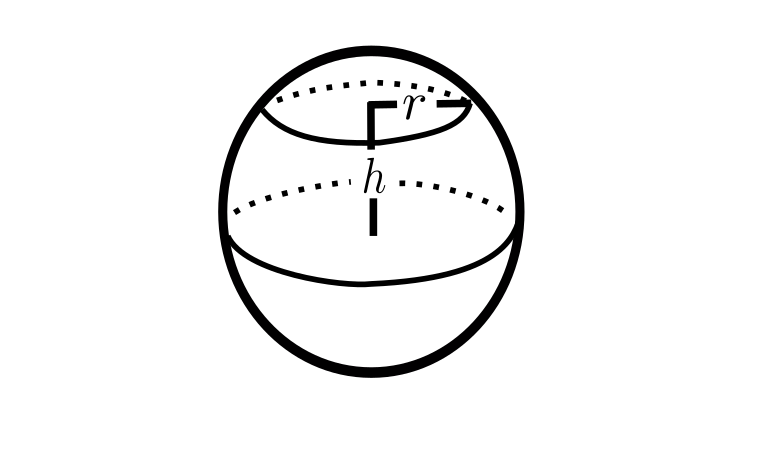
\includegraphics[width=.25\textwidth]{curvature/geodesic}
	\caption{Computing the geodesic curvature.}
	\label{fig:geodesic}
\end{figure}



\noindent \textbf{Exercises}


\begin{enumerate}
	\item Given the curve $\gamma(t)=(t,t^2)$ for $t\in[-1,1]$ compute 
	the radius of the osculating sphere at $t=0.$
	
	\item Given a curve $\gamma(t)$, if we traverse $\gamma(t)$ at unit speed,
	show that the tangent vector is orthogonal to the second derivative vector.
	
	\item 
	
\end{enumerate}

\pagebreak